\documentclass[12pt]{book}
\usepackage[utf8]{inputenc}
\usepackage{graphicx}
\usepackage{amsmath,amsfonts}
\usepackage{algorithm}
\usepackage{algorithmic}
\usepackage{array}
\usepackage[caption=false,font=normalsize,labelfont=sf,textfont=sf]{subfig}
\usepackage{setspace}
\usepackage{float}
\usepackage{textcomp}
\usepackage{stfloats}
\usepackage{url}
\usepackage{verbatim}
\usepackage{cite}
\usepackage{ragged2e}
\usepackage{url}
\setlength{\marginparwidth}{2.0cm} 
\usepackage[colorinlistoftodos]{todonotes}
\usepackage{afterpage}
\usepackage{acronym}
\usepackage[font=small]{caption}
\usepackage[hidelinks]{hyperref}
\usepackage{fancyhdr}
\pagestyle{fancy}
\setlength{\headheight}{14.5pt}
\addtolength{\topmargin}{-2.5pt}
\fancyhead{}
\fancyhead[LE,RO]{\thepage}
\fancyhead[LO,RE]{\slshape \leftmark}
\fancyfoot{}
\renewcommand{\chaptermark}[1]{}
\renewcommand{\sectionmark}[1]{\markboth{\thesection\ #1}{\thesection\ #1}}
\renewcommand{\subsectionmark}[1]{}

\fancypagestyle{plain}{%
  \fancyhead{}
  \fancyhead[LE,RO]{\thepage}
  \fancyfoot{}
  \renewcommand{\headrulewidth}{.6pt}
}

\newcommand{\zj}[1]{\textcolor{orange}{#1}}
\newcommand{\fmg}[1]{\textcolor{blue}{#1}}
\newcommand\blankpage{%
    \null
    \thispagestyle{empty}%
    \addtocounter{page}{-1}%
    \newpage
    \pagenumbering{gobble}% Suppress page numbering
}

% Set page margins
\usepackage[a4paper,margin=3.0cm]{geometry}


\DeclareMathOperator*{\argmax}{arg\,max}

\begin{document}

\begin{titlepage}
\begin{center}
\vspace*{3ex}
\textbf{\Huge Thesis}\\[2ex]
\textbf{\Huge Title}\\[2ex]
\textbf{\Huge of Your}\\[2ex]
\textbf{\Huge Work}\\[14ex]
\textbf{\large A thesis submitted in partial fulfilment}\\[1ex]
\textbf{\large of the requirement for the degree of Doctor of Philosophy}\\
[7ex]
\textbf{by}\\
[7ex]
\textbf{\LARGE Your name}\\
\vfill
\textbf{\LARGE June 2023}\\
\vfill

\includegraphics[width=0.8\textwidth]{logo.png}
\end{center}
\end{titlepage}

%\blankpage % Inserts a completely blank page

%\tableofcontents
\blankpage
\thispagestyle{empty} % Remove page number

\begin{center}
    \vspace*{\fill}
    \begin{quote}
    \textbf{In 1939, George Bernard Dantzig mistook two problems written on the blackboard as homework. He found the problems to be more challenging than normal. Despite their difficulty, he solved them. Those problems turned out to be open mathematical problems in statistics. This resulted in one of the shortest PhD theses ever.}
    \end{quote}
    \vspace*{\fill}
\end{center}

\blankpage
\blankpage

%\onehalfspacing %uncomment this if you need one-a-half line spacing from here...
\frontmatter 
\chapter*{Abstract}
\addcontentsline{toc}{chapter}{Abstract}

\ac{RL} Your abstract


\chapter*{Dedication}
\addcontentsline{toc}{chapter}{Dedication}

To my dearest wife,
\\

You have been my main support ....
\\


\noindent To my dear baby,
\\

As I write this dedication....
\\

\noindent To my dear mom,
\\

You were my first inspiration and my greatest supporter.....
\\

\noindent To my loving dad,
\\

You have been my constant source of guidance....


\chapter*{Declaration}
\addcontentsline{toc}{chapter}{Declaration}
%\textbf{\large Declaration}

This thesis is the result of my own independent work, except where otherwise stated,
and the views expressed are my own. Other sources are acknowledged by explicit
references. The thesis has not been edited by a third party beyond what is permitted
by Cardiff University's Use of Third Party Editors by Research Degree Students
Procedure.\\[2ex]
Signed \textbf{Your name} \ (candidate) \hspace*{10em}\\[1ex]
Date\ \ \ \ \ \textbf{22/July/2023} \hspace*{18em}
\vfill

\noindent\textbf{\large Statement 1}\\[1ex]
This thesis is being submitted in partial fulfilment of the requirements for the degree of PhD.\\[2ex]
Signed \textbf{Your name} \ (candidate) \hspace*{10em}\\[1ex]
Date\ \ \ \ \ \textbf{22/July/2023} \hspace*{18em}
\vfill

\noindent\textbf{\large Statement 2}\\[1ex]
This work has not been submitted in substance for any other degree or award at this
or any other university or place of learning, nor is it being submitted concurrently for
any other degree or award.\\[2ex]
Signed \textbf{Your name} \ (candidate) \hspace*{10em}\\[1ex]
Date\ \ \ \ \ \textbf{22/July/2023} \hspace*{18em}
\vfill

\noindent \textbf{\large Statement 3}\\[1ex]
I hereby give consent for my thesis, if accepted, to be available on the University’s
Open Access repository (or, where approved, to be available in the University's
library and for inter-library loans), and for the title and summary to be made available
to outside organisations, subject to the expiry of a University-approved bar on
access if applicable.\\[2ex]
Signed \textbf{Your name} \ (candidate) \hspace*{10em}\\[1ex]
Date\ \ \ \ \ \textbf{22/July/2023} \hspace*{18em}
\vfill

%%%%%%%%%%%%%%%%%%%%%%%%%%%%%%%%%%%%%%%%%%%%%%%%%%%%%%%%%%%%%%%%%%%%%%%%%%%%%%%%%%%%%%

\chapter*{Acknowledgements}
\addcontentsline{toc}{chapter}{Acknowledgements}

I would like to thank ...

\hfill

\noindent I am also grateful to...
\hfill

\noindent I would like to express my gratitude to ....

\hfill

\noindent I would like to thank my family ...



\tableofcontents

\listoffigures
\addcontentsline{toc}{chapter}{List of Figures}

\listoftables
\addcontentsline{toc}{chapter}{List of Tables}

\listofalgorithms
\addcontentsline{toc}{chapter}{List of Algorithms}

\chapter*{List of Acronyms} 
\addcontentsline{toc}{chapter}{List of Acronyms}

\begin{acronym}
\acro{AI}{Artificial intelligence}
\acro{RL}{Reinforcement learning}
\acro{HRI}{Human-robot interaction} 
\end{acronym}

\chapter*{List of Publications}
\addcontentsline{toc}{chapter}{List of Publications}


The work introduced in this thesis is based on the following publications:

\begin{itemize} 

\item \textbf{Your name} et al. Best paper ever in the entire universe. IEEE Transactions on Neural Networks and learning systems. 2023



\end{itemize}

\noindent Other publications:

\begin{itemize} 

\item \textbf{Your name} et al. Best paper ever in the entire universe. IEEE Transactions on Neural Networks and learning systems. 2023


\end{itemize}

\mainmatter
\onehalfspacing
\chapter{Introduction}
\label{sec:chapter1}
\ac{AI} has significantly evolved over the years~\cite{shao2019survey}.....

\section{Motivation}

The performance of an \ac{AI} agent depends on...


To summarise, \ac{AI} performance relies on ...

\section{Research questions}

The following research questions will be addressed in this thesis:

\begin{itemize}
    \item How does ...?
    \item How to ...?
    \item Can ...?
    \item Is ...?
    \item Is \ac{AI} ...?
\end{itemize}

A detailed examination based on a literature review, experiments, and analysis will be conducted for each one of the questions above. These questions answers hold the potential to provide helpful information about the benefits and limitations of using affordances for training RL agents, as well as understanding the factors required to carry out ... 

\section{Aim and Objectives}

This thesis aims to investigate ..... To achieve this aim, the following objectives are pursued: 

\begin{itemize}
    \item To investigate ...
    \item To develop ...
    \item To develop ...
\end{itemize}

By pursuing these objectives, this thesis aims to contribute to ...

\section{Outline}

This outline presents a concise summary of the thesis' content comprised of six chapters, aiming to provide a clear overview of the research presented in the following chapters.\\


\noindent\textbf{Chapter \ref{sec:chapter2}} introduces relevant literature in ...\\

\noindent\textbf{Chapter \ref{sec:chapter3}}  introduces ....\\

\noindent\textbf{Chapter \ref{sec:chapter4}} introduces ...\\

\noindent\textbf{Chapter \ref{sec:chapter5}} presents .... \\

\noindent\textbf{Chapter \ref{sec:chapter6}} concludes the thesis by summarising the main contributions and achievements of this research work. In addition, the limitations and challenges of the approaches developed in this thesis are discussed, and propose future research directions.\\ 

\noindent Overall, this thesis aims to contribute to the ongoing efforts to improve ....

\chapter{Literature review}
\label{sec:chapter2}

In the field of ..... The rest of the chapter is organised as follows, section~\ref{chap2:rl_overview} introduces relevant concepts in \ac{RL}. Then, section~\ref{chap2:context_rl} explores how contextual information is involved in current state-of-the-art approaches. Followed by section~\ref{chap2:rl_robotics} that focuses on robotic applications, more concisely, on the use of \ac{RL} for the manipulation of rigid and deformable objects. Finally, the main findings of the literature review are discussed in section~\ref{chap2:discussion} and summarised in section~\ref{chap2:summary}.   

\section{Reinforcement learning overview}
\label{chap2:rl_overview}


\subsection{The Bellman optimality equation}

The Bellman optimality equation expresses the expected maximum or total reward that can be achieved from a given state based on the value function (Eq.~\eqref{C2eq:04}). The equation defines the relationship between the value of a state and the values of its neighbouring states. The Bellman optimality equation of the value function is given by the following:

\begin{equation}\label{C2eq:04}
V^{*}(s)=\max\limits_{a}\sum_{s'}^{}P(s'| s,a)(R(s,a,s')+\gamma V^{*}(s'))
\end{equation}


\section{Context and RL}
\label{chap2:context_rl}



\section{Reinforcement learning in robotics}
\label{chap2:rl_robotics}
This section introduces relevant research in the field of robotics and \ac{RL}, where classical and RL approaches are applied to solve \ac{HRI} problems and manipulation tasks of rigid and deformable objects.

\subsection{Why reinforcement learning in robotics?}
\label{chap2:rl_robotics_why}


\subsection{Robotic manipulation of rigid objects with reinforcement learning}
\label{chap2:rl_robotics_rigid}



\subsection{Reinforcement learning in human-robot interaction}
\label{chap2:rl_robotics_hri}


\subsection{Robotic manipulation of deformable objects with reinforcement learning}
\label{chap2:rl_robotics_deformable}

\section{Discussion}
\label{chap2:discussion}

This section delves into a detailed analysis of the advantages and disadvantages of ....

Additionally, current research endeavours have been made to explore the implementation of ...

Despite the advantages of the discussed approaches, there are still challenges related to ...

\begin{itemize}
    \item Lack of ...  
\end{itemize}


\section{Summary}
\label{chap2:summary}

This chapter has provided valuable insights into the implementation of ...

This literature review has also identified several gaps in the current knowledge of ....

To address these gaps, an incremental approach is followed in this thesis...

\chapter{Title chapter 3} 
\label{sec:chapter3}
\section{Introduction}
\label{C3sec:introduction}




\chapter{Title chapter 4} 
\label{sec:chapter4}


\begin{figure*}
\centering
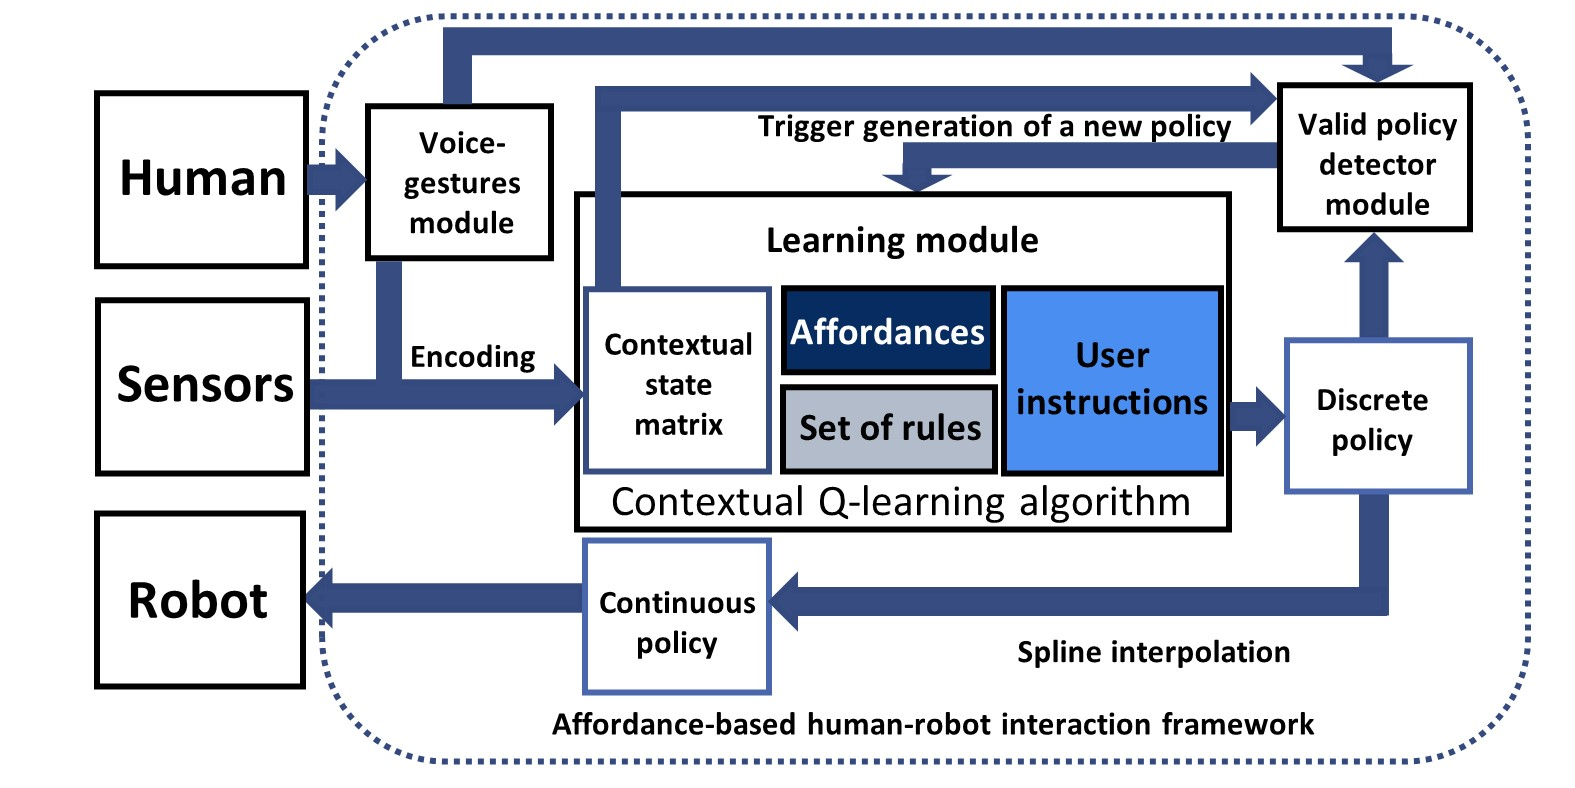
\includegraphics[width=5.0in]{C4/cql_framework.jpg}
\caption{Proposed framework. }
\label{C4fig:framework}
\end{figure*}



\chapter{Title chapter 5} 
\label{sec:chapter5}
\input{C5/chapter5}

\chapter{Contributions, conclusions, and future work} 
\label{sec:chapter6}
This chapter concludes the study undertaken in this work. Section~\ref{sec5:contributions} focuses on highlighting the main contributions of this thesis. The findings and key takeaways are presented in Section~\ref{sec5:conclusions}, while recommendations for future research directions are discussed in Section~\ref{sec5:future}.

\section{Contributions}
\label{sec5:contributions}

The contributions of this thesis are summarised as follows:

\begin{itemize}
\item First contribution ...
\end{itemize}

\section{Conclusions}
\label{sec5:conclusions}

In conclusion, this thesis has explored the impact of ...

Overall, this thesis makes a valuable contribution to ...
\section{Future work}
\label{sec5:future}

The research conducted in this thesis has provided valuable insight into the fields of ....

\begin{itemize}

\item Investigation of ...
    
\end{itemize}



%\bibliographystyle{plain}
%\bibliographystyle{agsm}
\bibliographystyle{unsrt}
\bibliography{bibliography}

\end{document}
